\chapter{Chapter 5:  Assessing coastal vulnerability using directional spectral
wave climate: Coastal Vulnerability Index} 
\label{chapter5}


\section{Introduction}
\label{c5_Introduction}

Coastal vulnerability, referring to the assessment of places and lives in
coastal regions that are susceptible to the impacts of coastal hazards, is a key
concept in coastal environment \citep{bevacqua_coastal_2018}. Coastal regions
are among the most developed and densely populated areas globally, with over
3.34 billion people—approximately 44.6\% of the world's population—residing
within 150 kilometers of a coastline by 2018 \citep{cosby_accelerating_2024}.
However, coastal regions are also highly dynamic and vulnerable to severe
hazardous events, which poses significant threats to coastal physical,
economical, biological and social aspects
\citep{bevacqua_coastal_2018,kantamaneni_assessing_2018}. For example, coastal
zones are extremely sensitive to sea-level rise, which can trigger multiple
coastal hazards, including coastal flooding, shoreline erosion, infrastructure
failure and saltwater intrusion \citep{gornitz_global_1991}. These hazards can
pose significant risks to both natural ecosystems and human settlements in
coastal areas, even causing casualty. In Lake Michigan, a rising lake level has
been observed since 2014, which increases the risks of the coastal
\citep{gronewold_hydrological_2016,zoet_analysis_2017,troy_rapid_2021}. Facing
increasing threats, significant resources have been committed to construct,
maintain, and repair coastal structures, with approximately \$2.9 billion
invested between 1959 and 1990 \citep{angel_large-scale_1995}. Simultaneously,
numerous projects have been launched to assess coastal vulnerability and develop
strategies for mitigating potential risks, nevertheless, most of these are based
on qualitative assessment \citep{salus_addressing_2024}. Therefore, a
significant knowledge gap remains: the development of a quantitative approach
tailored to the unique geological and hydraulic conditions of Lake Michigan.

The Coastal Vulnerability Index (CVI) is a widely used approach for quantifying
the potential impacts of coastal hazards and assessing coastal vulnerability.
\citet{gornitz_global_1991} first introduced CVI in the early 1990s to evaluate
coastal hazards associated with sea-level rise. The original Coastal
Vulnerability Index (CVI) framework included seven key variables: relief, rock
type, landform, vertical movement, shoreline displacement, tidal range, and wave
height. These variables collectively account for factors influencing flooding
risk, resistance to erosion, and hydrodynamic processes, providing a
comprehensive assessment of coastal vulnerability \citep{shaw_sensitivity_1998}.
Each variable was quantified using an integer scale from 1 to 5, representing
increasing levels of risk and vulnerability. The CVI was then calculated as the
square root of the product of the seven ranked variables, divided by the total
number of variables, providing a quantitative measure of overall coastal
vulnerability \citep{koroglu_comparison_2019}. This framework has been adopted
by numerous studies, often with minor adaptations for the ranking criteria to
better suit specific regional or environmental contexts
\citep[\eg][]{royo_rapid_2016,shaw_sensitivity_1998,thieler_national_2000}.
Furthermore, the Fiscal Coastal Vulnerability Index (FCVI) was introduced to
account for economic vulnerability along coastlines by integrating factors such
as commercial impacts, population density, and the economic value of coastal
infrastructure \citep{kantamaneni_assessing_2018}.In summary, significant
efforts have been made to develop vulnerability indices that incorporate the
impacts of sea-level rise, economic values and wave impacts.  Nevertheless, the
Coastal Vulnerability Index (CVI), typically based on wave height, is inadequate
for Lake Michigan as it overlooks the complex influences of the directional
spectral wave climate on coastal vulnerability in Lake Michigan.

Directional spectral wave climate, characterized by the directionality and
modality of wind waves spectrum, are essential factors contributing to coastal
vulnerability, as they can imply the risks of various coastal hazards. Wave
directionality refers to the patterns of wave propagation directions, whereas
modality describes the distribution of wave energy across different frequencies
\citep{coates_beach_1998,wiggins_coastal_2019,wiggins_regionally-coherent_2019}.
Both directionality and modality can contribute to coastal erosion by
influencing sediment transport patterns and dynamics. For example, wave
bidirectionality, a special type of wave directionality characterized by waves
approaching from two opposing or oblique directions, is recognized as a
significant contributor to directions of the longshore sediment transport
\citep{seymour_longshore_2019}. Bidirectional waves can generate opposing
longshore sediment transport, which can result in imbalances in sediment budgets
within a littoral cell, ultimately contributing to severe coastal erosion
\citep{davidson-arnott_wave_1980,galal_influence_2011,hapke_review_2010}.
Meanwhile, bidirectional longshore sediment transport can also lead to beach
rotation in embayment beach
\citep{klein_short-term_2002,wiggins_regionally-coherent_2019}. Coastal erosion
and rotation can leave coastal community and structures vulnerable to damage
from extreme wave climate \citep{wiggins_coastal_2019}. Similarly, wave modality
reflects sea states by representing the distribution of wave energy across
different frequencies, which also imply the patterns and dynamics of the
nearshore sediment transport. For example, high-frequency wave modality, often
associated with swell, can transport more sediment than wind-sea over longer
distances and contribute to broader-scale coastal reshaping due to the fact that
swell has comparatively shorter wave period and higher wave energy
\citep{george_nearshore_2020}. Due to this characteristics, high-frequency
modality or swell is considered as stronger contributor to broader-scale coastal
changing \citep{basaran_effect_2021}. To date, both wave directionality and wave
modality contribute to coastal vulnerability by indicating severe coastal hazard
including coastal erosion and beach rotation. 

Despite the fact that directional spectral wave climate is important to coastal
vulnerability as it implies the coastal erosion and rotation, few studies have
tried to incorporate these mechanisms into the framework of CVI in the past. For
coastal erosion, the Beach Vulnerability Index (BVI), a specialized variant of
the CVI, was introduced to focus on coastal beach erosion within nearshore
systems \citep{alexandrakis_holistic_2014}. BVI incorporates key factors such as
nearshore longshore sediment transport, nearshore cross-shore sediment
transport, and wind-driven sediment transport, offering a more detailed
assessment of coastal vulnerability related to sediment budgets and shoreline
stability. Nevertheless, BVI does not incorporate the directional impact of wave
climate but assuming a bulk sediment transport direction. For coastal rotation,
the Rotational Index (RI) and Wave Power Directionality Index (WDI) have been
proposed to quantify the intensity of beach rotation responses and the degree of
wave directionality, respectively
\citep{wiggins_coastal_2019,wiggins_regionally-coherent_2019}. Although these
two indices are correlated with the process of coastal rotation, they are not
designed as indicators within a coastal vulnerability framework and, therefore,
cannot directly represent the risk associated with coastal rotation. In summary,
the BVI, RI, and WDI can be incorporated into the Coastal Vulnerability Index
(CVI) framework to better capture the complex processes of coastal erosion and
rotation driven by Lake Michigan's directional spectral wave climate.
Consequently, a revised CVI tailored to these dynamics is essential for
accurately assessing coastal vulnerability in Lake Michigan.

The objective of this study is to develop an innovative index – coastal 
vulnerability index (CVI) - to assess the vulnerability of beaches, considering
the directional spectral wave climate. RVI will be developed based on the
framework of the CVI in 1991 \citep{gornitz_global_1991}, with advancement of innovative
knowledge about coastal rotation caused by directional spectral wave climate.
This study hypothesizes that RVI provides a better assessment of coastal
vulnerability considering the beach rotation caused by directional spectral wave
climate. To support this hypothesis, several research questions are proposed
below.

\section{Study sites}
\label{c5_Study sites}

\begin{figure}[htbp]
  \centering
  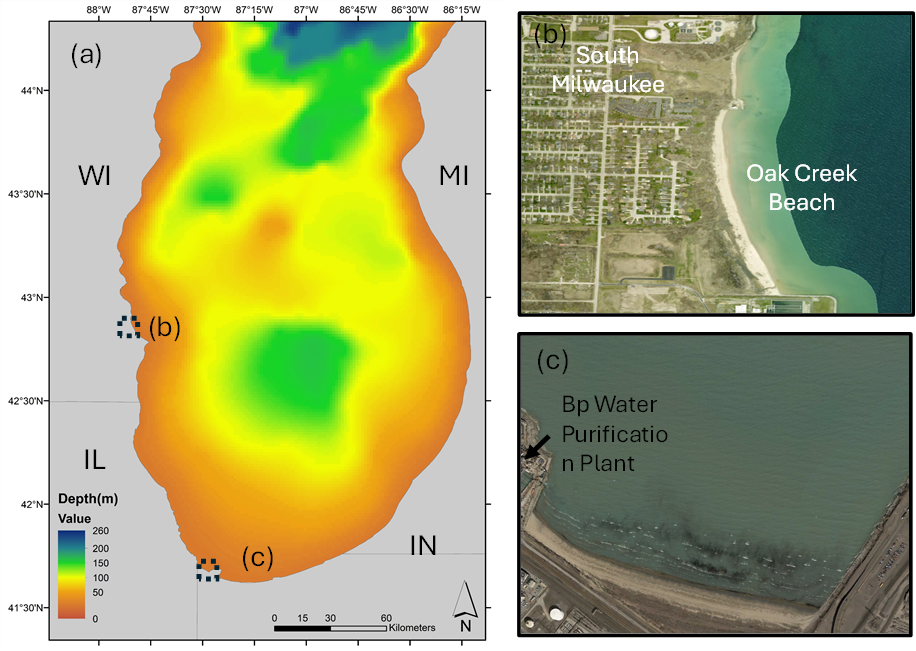
\includegraphics[width=1\textwidth]{chapter5/resources/study_sites.png}
  \caption{Study sites. (a) locations of two head bay beaches, (b) Oak Creek
  Beach located in southern Milwaukee, Wisconsin and (c) Whiting Lakefront Park
  beach located in Indiana}
  \label{fig:c5_study_sites}
\end{figure}

Study sites are located along the southern coast of Lake Michigan (see Figure
\ref{fig:c5_study_sites}a). Lake Michigan, one of North America's five Great
Lakes, is a glacially formed freshwater basin bordered by the states of
Illinois, Indiana, Michigan, and Wisconsin. It is the second-largest Great Lake
by volume and the third-largest by surface area, with a roughly elongated
north-south orientation.  The lake spans approximately 494 kilometers in length
and 190 kilometers at its widest point. The basin is asymmetrical, featuring a
steep western shoreline contrasted by gentler slopes on the eastern side, with a
maximum depth of about 281 meters.

There are two headland bay beaches selected in the study area for their
representative wave climates. The first beach is located in Oak Creek Park of
southern Milwaukee, Wisconsin, which is presented in Figure
\ref{fig:c5_study_sites}b. The total length of Oak Creek beach is approximately
0.5 miles (800 meters) in the orientation of north-south direction. The wave
directionality in the Oak Creek Park is a typical bidirectional wave, that waves
come from two opposite directions (see Figure \ref{fig:c5_sites_climate}a). The
second site is located in Whiting Beach in Indiana, where the domiant wave comes
from the northern direction (see Figure \ref{fig:c5_study_sites}b). The
significant wave height in Oak Creek is slightly larger than the wave height in
Whiting Beach, nevertheless, they have a similar inter-annual trend, as shown in
Figure \ref{fig:c5_sites_climate}c.  

\begin{figure}[htbp]
  \centering
  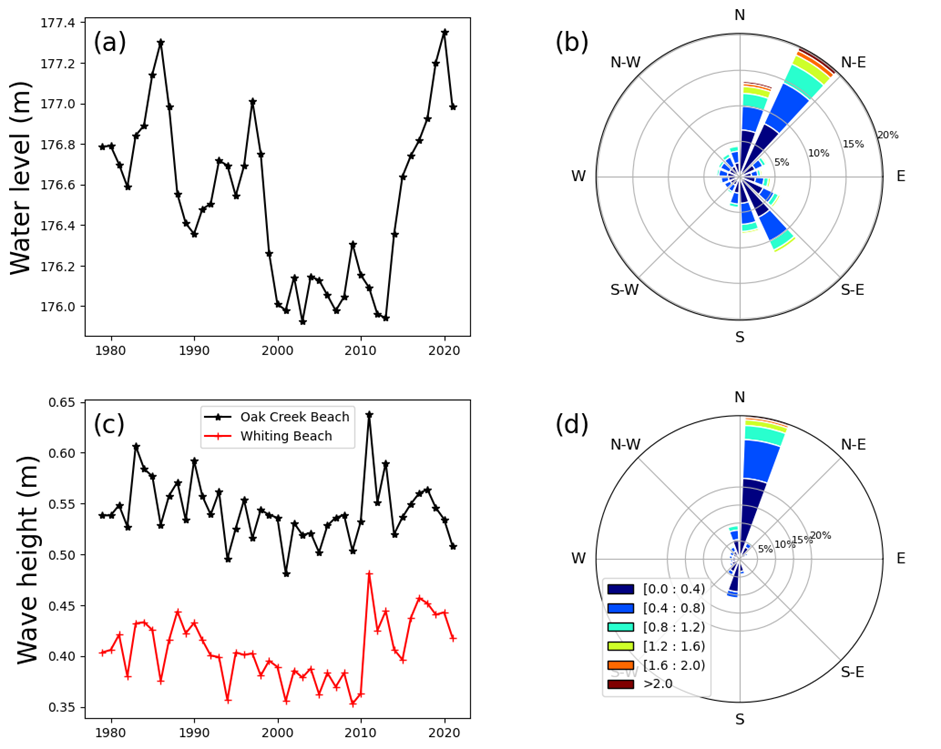
\includegraphics[width=1\textwidth]{chapter5/resources/cites_climates.png}
  \caption{Climatology in study sites. (a) water level and (c) wave height in southern Lake Michigan. (b)
  and (d) are the wave rose in Oak Creek Beach and Whiting Beach, respectively}
  \label{fig:c5_sites_climate}
\end{figure}

\section{Methods}
\label{c5_Methods}

\subsection{Formulation of coastal vulnerability index}
\label{Formulation of coastal vulnerability index}

\begin{figure}[htbp]
  \centering
  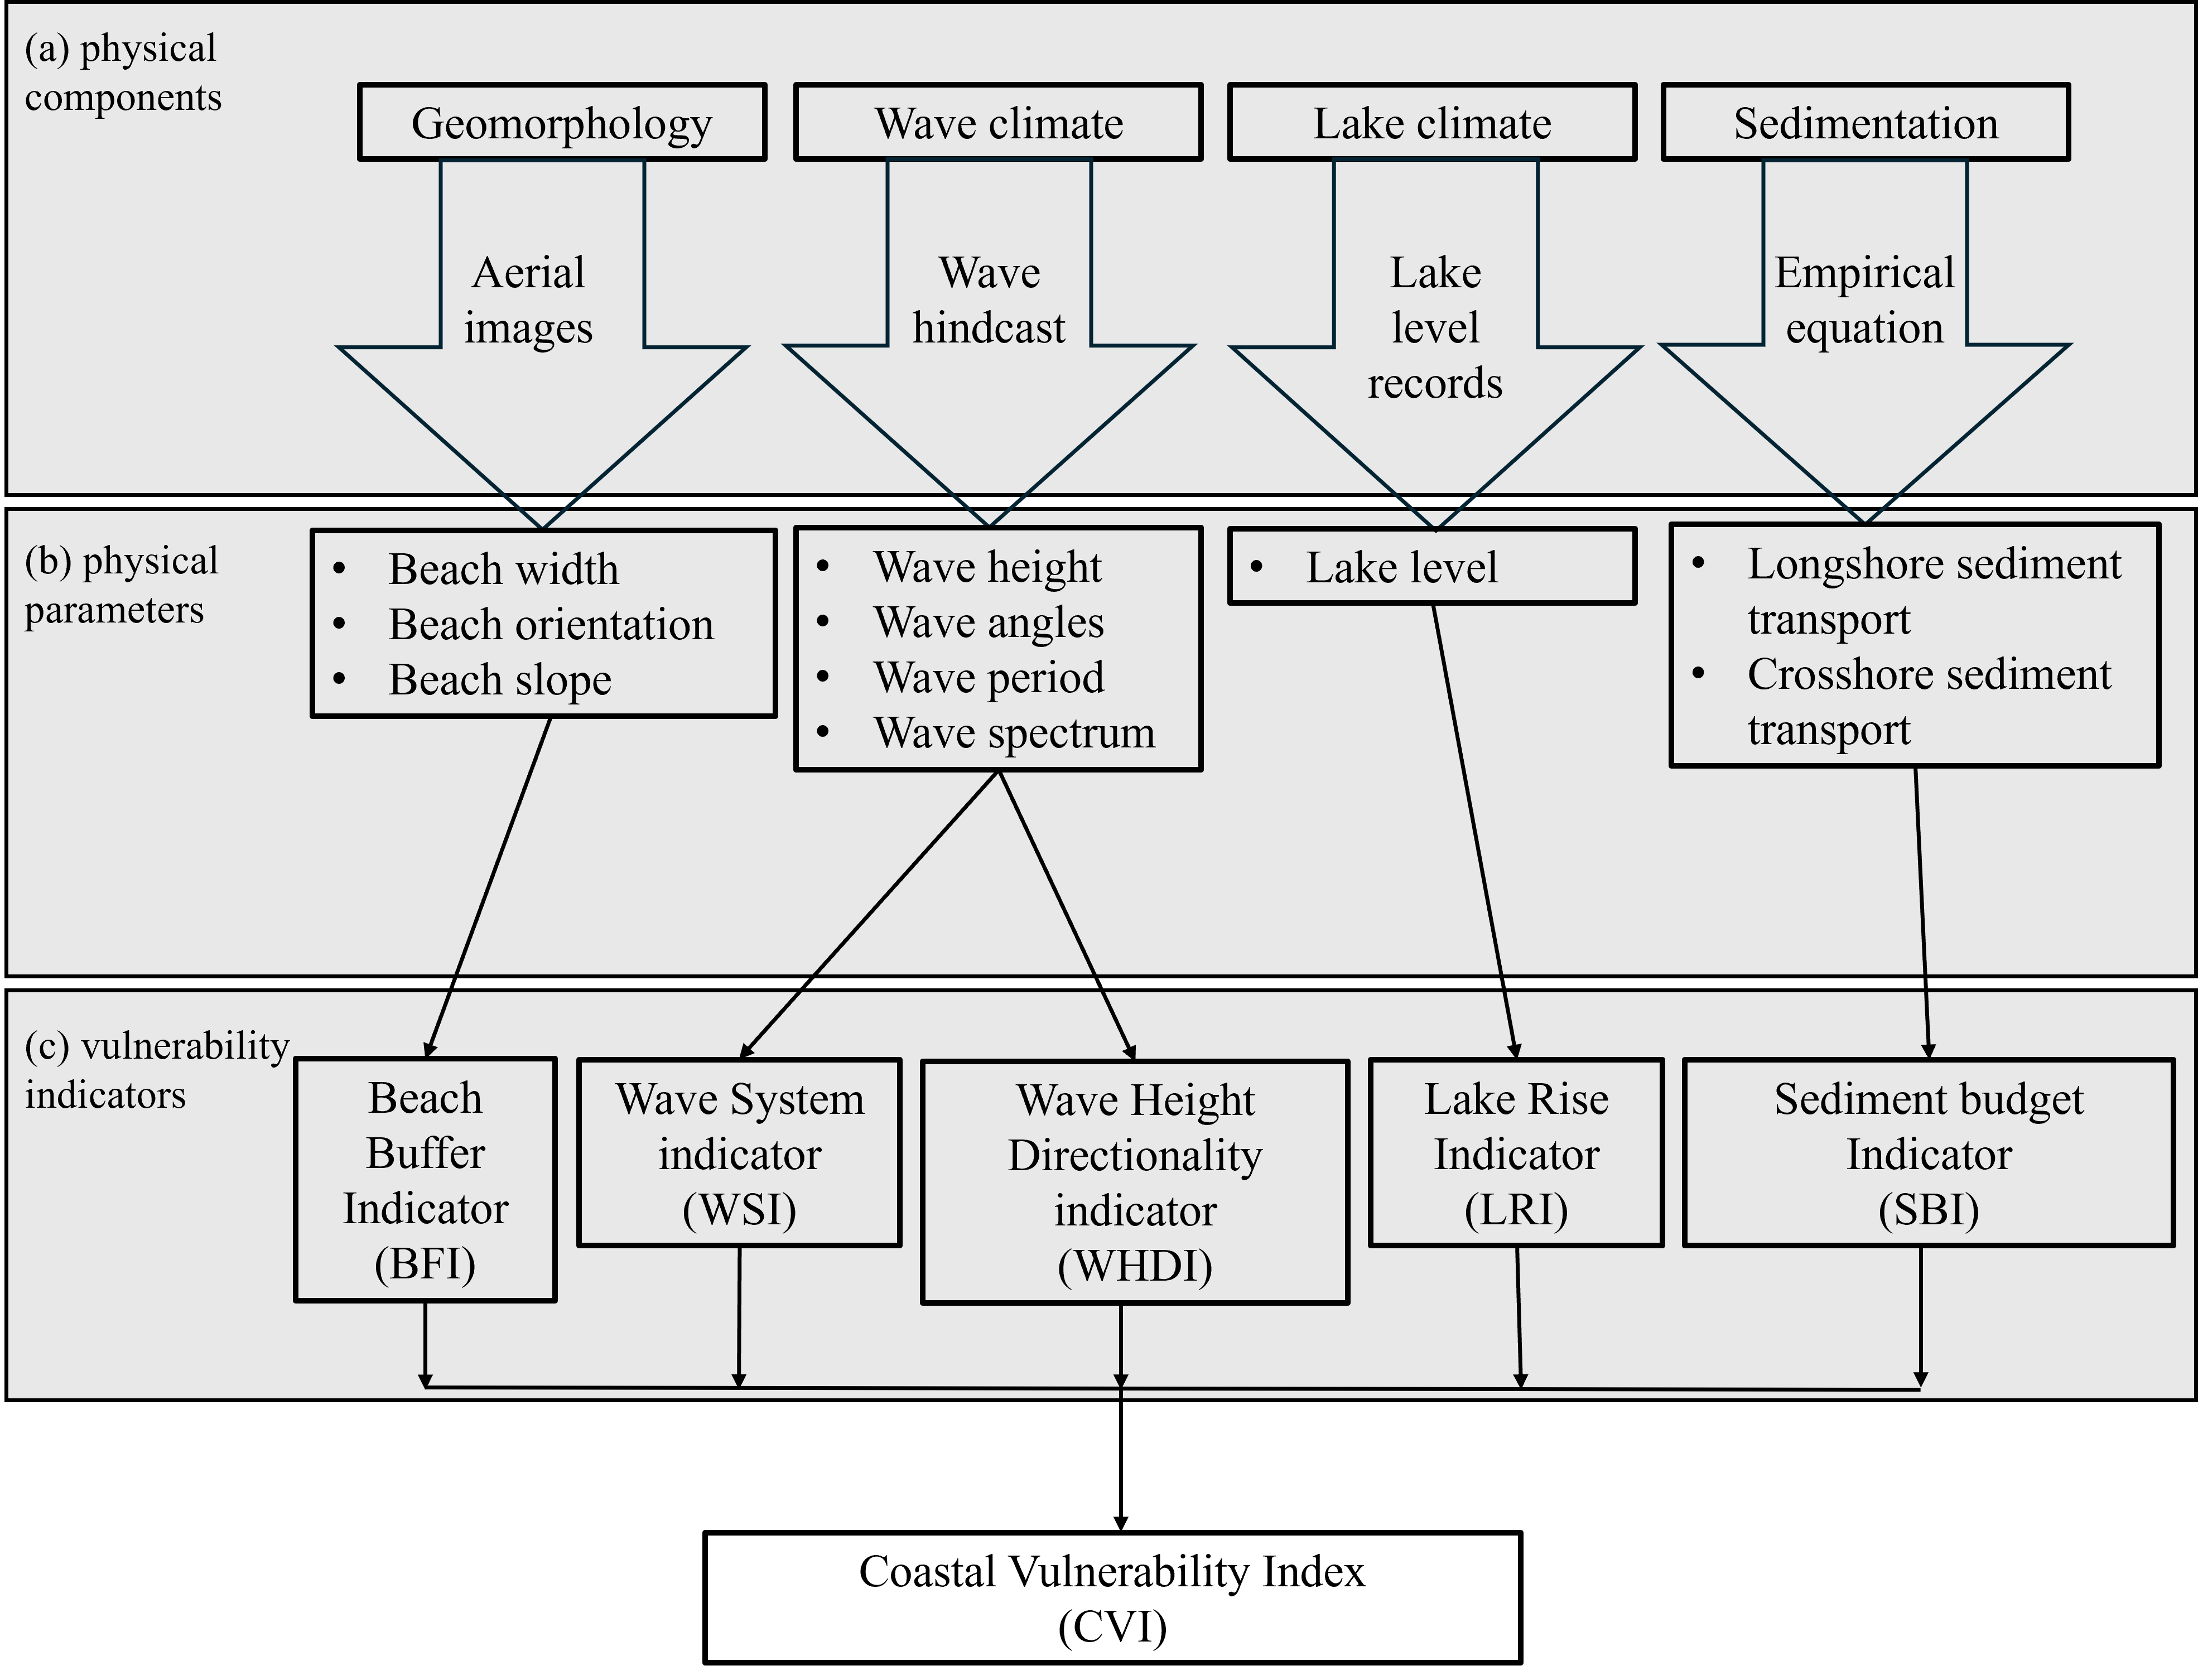
\includegraphics[width=1\textwidth]{chapter5/resources/c5_methods_graph.png}
  \caption{formulation of coastal vulnerability index from (a) physical
  components (b) parameters to (c) indicators.}
  \label{fig:c5_method_cvi}
\end{figure}

Our coastal vulnerability index (CVI) follows the framework of original CVI
proposed by \citet{gornitz_global_1991}. Nevertheless, to reflect Lake
Michigan’s climate of wave and water level, there are multiple modifications for
the components of CVI we proposed. In General, four major components were
discussed in CVI (see Figure \ref{fig:c5_method_cvi}a): geomorphology, wave
climate, lake level climate, and sedimentation. Geomorphology refers to the
shape and change of coastal landforms, specifically, the coastal sandy beach in
this study. Geomorphology is considered as one component of coastal
vulnerability as it offers a protective buffer to coastal hazard. Wave climates
are the characteristics of long-term wave statistics such as wave heights and
wave direction. Lake level climate reflects the fluctuation of water level. In
Lake Michigan, a periodic water level rise and fall were recorded by decades.
Both wave and water level are considered as driver of coastal hazard which
jeopardize the coastal vulnerability. The sedimentation is regarded as the
suspension and transportation of nearshore sediment. Longshore sediment
transport, one component of the sedimentation, is also contributing to coastal
erosion, which impacts the coastal vulnerability.

These components can be quantified by several physical parameters (see Figure 
\ref{fig:c5_method_cvi}b). For instance, beach width serves as a measure of the
buffer protection provided by the beach, with larger beach widths indicating
greater coastal resilience and lower vulnerability. The beach slope is another
critical parameter influencing beach vulnerability, as it is closely associated
with the impacts of waves and water level variations \citep{swenson_bluff_2006}.
Wave parameters, including significant wave height, wave direction, wave period
and wave spectrum, will be considered as parameters for wave climates. For lake
level climates, lake level variation is utilized to quantify fluctuations in
Lake Michigan's water levels. Last but not least, the rate of the longshore
sediment transport and crosshore sediment transport could be the parameters for
the sedimentation. Table \ref{Summary of data sources} summarizes the data
sources for these parameters.

\begin{table}[htbp]
\centering
\caption{Summary of data sources}
\label{Summary of data sources}
\begin{tabular}{|p{3cm}|p{4cm}|p{4cm}|p{4cm}|}
\hline
\textbf{Physical parameters} & \textbf{Data source} & \textbf{Date} & \textbf{Resolution} \\ \hline
Shoreline position & NAIP aerial image & 2008-2020 & 0.3 m \\ \hline
Beach slope & USACE NCMP Topobathy Lidar & 2020 & 1 m (horizontal), 0.1 m (vertical) \\ \hline
Wave height, angle, period & WIS stations 94005 and 94046 & 2008-2020 & Hourly \\ \hline
Water level & NOAA meteorology stations 9087057 and 9087044 & 2008-2020 & Hourly \\ \hline
\end{tabular}
\end{table}


With the proposed parameters, five vulnerability indicators were developed with
the combinations of these parameters, as shown in Figure
\ref{fig:c5_method_cvi}c. Beach buffer indicator ($BFI$) reflects the
vulnerability of beach erosion, which is modified index from 
\citet{wiggins_regionally-coherent_2019}.

\begin{equation}
    BFI = \frac{S}{WL}
\label{eq:eq5.1}
\end{equation}

Where $W$ represents the beach width at current position, $L$ is the longshore
distance of beach, and $S$ represents the beach slope at the position. The
second indicator is the Wave System Indicator ($WSI$), which indicates the
relative impact of wave system between wind-sea and swell. In our study, $WSI$
was computed by hourly WIS spectral data from 2008 to 2020. Here is the
definition of $WSI$.

\begin{equation}
    WSI = \frac{m_{0ws}}{m_{0tot}}
\label{eq:eq5.2}
\end{equation}

Where the $m_{0ws}$ is the zeroth order moment of wind-sea wave energy spectrum
and $m_{0tot}$ is the zeroth order moment of total wave energy spectrum.The
third parameter is the Wave height directionality indicator ($WHDI$) which
reflects the directionality of wave climate in Lake Michigan.  Here is the
definition.

\begin{equation}
    WHDI = \frac{|\sum H_{s1}-\sum H_{s2}|}{\sum H_{s1}+\sum H_{s2}}
\label{eq:eq5.3}
\end{equation}

where $H_{s1}$ and $H_{s1}$ represent wave heights weighted by significant wave
height at the two predominant wave directions. Unlike to previous method that
calculate the two dominant waves at two fixed directions
\citep{wiggins_coastal_2019,wiggins_regionally-coherent_2019}, the two
predominant directions were selected based on the orientation of beach
morphology as we define the left side of beach normal vector is the first
dominant direction and right side of beach normal vector is the second dominant
direction. The fourth indicator counts the impacts of water level and wave
actions, which is Lake Rise Indicator ($LRI$). 

\begin{equation}
    LRI = \frac{R + 0.068 H_b}{S}
\label{eq:eq5.4}
\end{equation}

Where $R$ stands for rise of lake level in meters, $H_b$ stands for the breaking
wave height, $S$ is the beach slope. The last indicator is Sediment Budget
Indicator ($SBI$), which rely on the Komar estimation of longshore sediment
transport rate.

\begin{equation}
    SBI = Q_{Komar} = 1.1 \rho g^{1.5} H_b^{2.5}\sin\alpha_b\cos\alpha_b
\end{equation}
\label{eq:eq5.5}

Where $Q_{Komar}$ is potential volumetric longshore sediment transport rate in
$m^3/day$, $\rho$ is water density ($g/cm^3$), $g$ is the gravitational
acceleration, $H_b$ is the breaking wave height and $\alpha_b$ is the breaking
wave angle.

\subsection{Coastal vulnerability index}
\label{Coastal vulnerability index}

\begin{figure}[htbp]
  \centering
  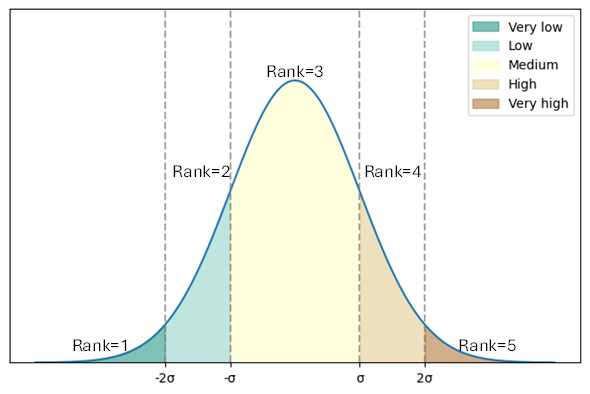
\includegraphics[width=1\textwidth]{chapter5/resources/five_ranks.png}
  \caption{Definition of five ranks based on normal distribution. $\alpha$ is the
  standard deviation to the total sets of beach segment in two study sites.}
  \label{fig:five_ranks}
\end{figure}

Since the five indicators have different physical meanings and magnitudes, their
values were standardized and converted into a rank of vulnerability ranging from
1 (very low) to 5 (very high). This ranking was determined using a standard
normal distribution applied to the dataset of 8 beach segments at Oak Creek
Beach and 12 beach segments at Whiting Beach, each spaced at 100-meter intervals
(see Figure \ref{fig:five_ranks}). Then, the overall coastal vulnerability index (CVI) is defined
as the square root of the product of ranks divided by the number of variables n.

\begin{equation}
    CVI = \sqrt{\frac{r_1*r_2*r_3*r_4*r_5}{5}}
\label{eq:eq5.6}
\end{equation}

Where the $r_1$ to $r_5$ are the ranks of five indicators for vulnerability,
respectively.

\subsection{Evaluation of index}
\label{Evaluation of index}
The performance of the Coastal Vulnerability Index (CVI), defined in Equation
\ref{eq:eq5.6}, was evaluated by comparing both the overall index and its
component subindices ($r_{1}$–$r_{5}$) with observed shoreline change. Following
established approaches in coastal vulnerability assessment
\citep[\eg][]{fuller2002bank,thieler2000national}, we used historical end-point
rate (EPR) estimates of shoreline erosion as the observational benchmark. At
Whitting Beach, EPRs were calculated for 2008–2013, 2013–2015, 2015–2018, and
the high-water interval of 2018–2020; at Oak Creek Beach, EPRs were computed for
2010–2012, 2012–2014, 2014–2016, and 2016–2018. To ensure comparability with the
CVI, the continuous EPR values were standardized and classified into five
ordinal categories, consistent with the CVI ranking scheme.  

To quantify the agreement between predicted CVI (and subindex) ranks and
observed erosion-rate ranks, we employed five complementary metrics commonly
used for ordinal data:

\begin{itemize}
  \item \textbf{Mean Absolute Error (MAE):}  
  \begin{equation}
    MAE = \tfrac{1}{N}\sum_{i=1}^{N} \lvert \hat{y}_i - y_i \rvert
  \end{equation}
  where $\hat{y}_i$ and $y_i$ are predicted and observed ranks, respectively.
  MAE reflects the average magnitude of misclassification and is easily
  interpretable on the 0–5 ranking scale; unlike RMSE, it does not overweight
  large errors \citep{Willmott2005,Chai2014}.
  
  \item \textbf{Root Mean Square Error (RMSE):}  
  \begin{equation}
  RMSE = \sqrt{\tfrac{1}{N}\sum_{i=1}^{N} \left(\hat{y}_i - y_i\right)^2}
  \end{equation}
  RMSE penalizes larger misclassifications more strongly than MAE and is useful
  when large deviations are of particular concern \citep{Chai2014,Willmott2005}.
  
  \item \textbf{Quadratic Weighted Kappa (QWK):} a chance-corrected agreement
  coefficient for ordinal categories \citep{Cohen1968}. Given observed ratings
  $O_{ij}$ and expected ratings $E_{ij}$ in the $k \times k$ confusion matrix,
  \begin{equation}
    \kappa_w = 1 - \frac{\sum_{i,j} w_{ij} O_{ij}}{\sum_{i,j} w_{ij} E_{ij}}
  \end{equation}
  where the quadratic weight is 
  $w_{ij} = \tfrac{(i-j)^2}{(k-1)^2}$. Larger values indicate stronger
  agreement, with qualitative interpretations (``slight,'' ``fair,''
  ``moderate,'' etc.) sometimes applied \citep{Landis1977}.
  
  \item \textbf{Spearman’s rank correlation ($\rho$):}  
  \begin{equation}
    \rho = 1 - \frac{5\sum_{i=1}^{N} d_i^2}{N(N^2-1)}
  \end{equation}
  where $d_i = \text{rank}(\hat{y}_i) - \text{rank}(y_i)$. This measures the
  strength of the monotonic association between predicted and observed ranks
  without assuming linearity \citep{Spearman1904}.
  
  \item \textbf{Kendall’s $\tau$:} defined as
  \begin{equation}
    \tau = \frac{C - D}{\tfrac{1}{2}N(N-1)}
  \end{equation}
  where $C$ and $D$ denote the numbers of concordant and discordant pairs,
  respectively. $\tau$ is often more conservative than $\rho$ in finite samples
  \citep{kendall_new_1938}.
\end{itemize}

\section{Results}
\label{c5_Results}

\subsection{Coastal vulnerability index at Oak Creek Beach}
\label{Coastal vulnerability index at Oak Creek Beach}

\begin{figure}[htbp]
  \centering
  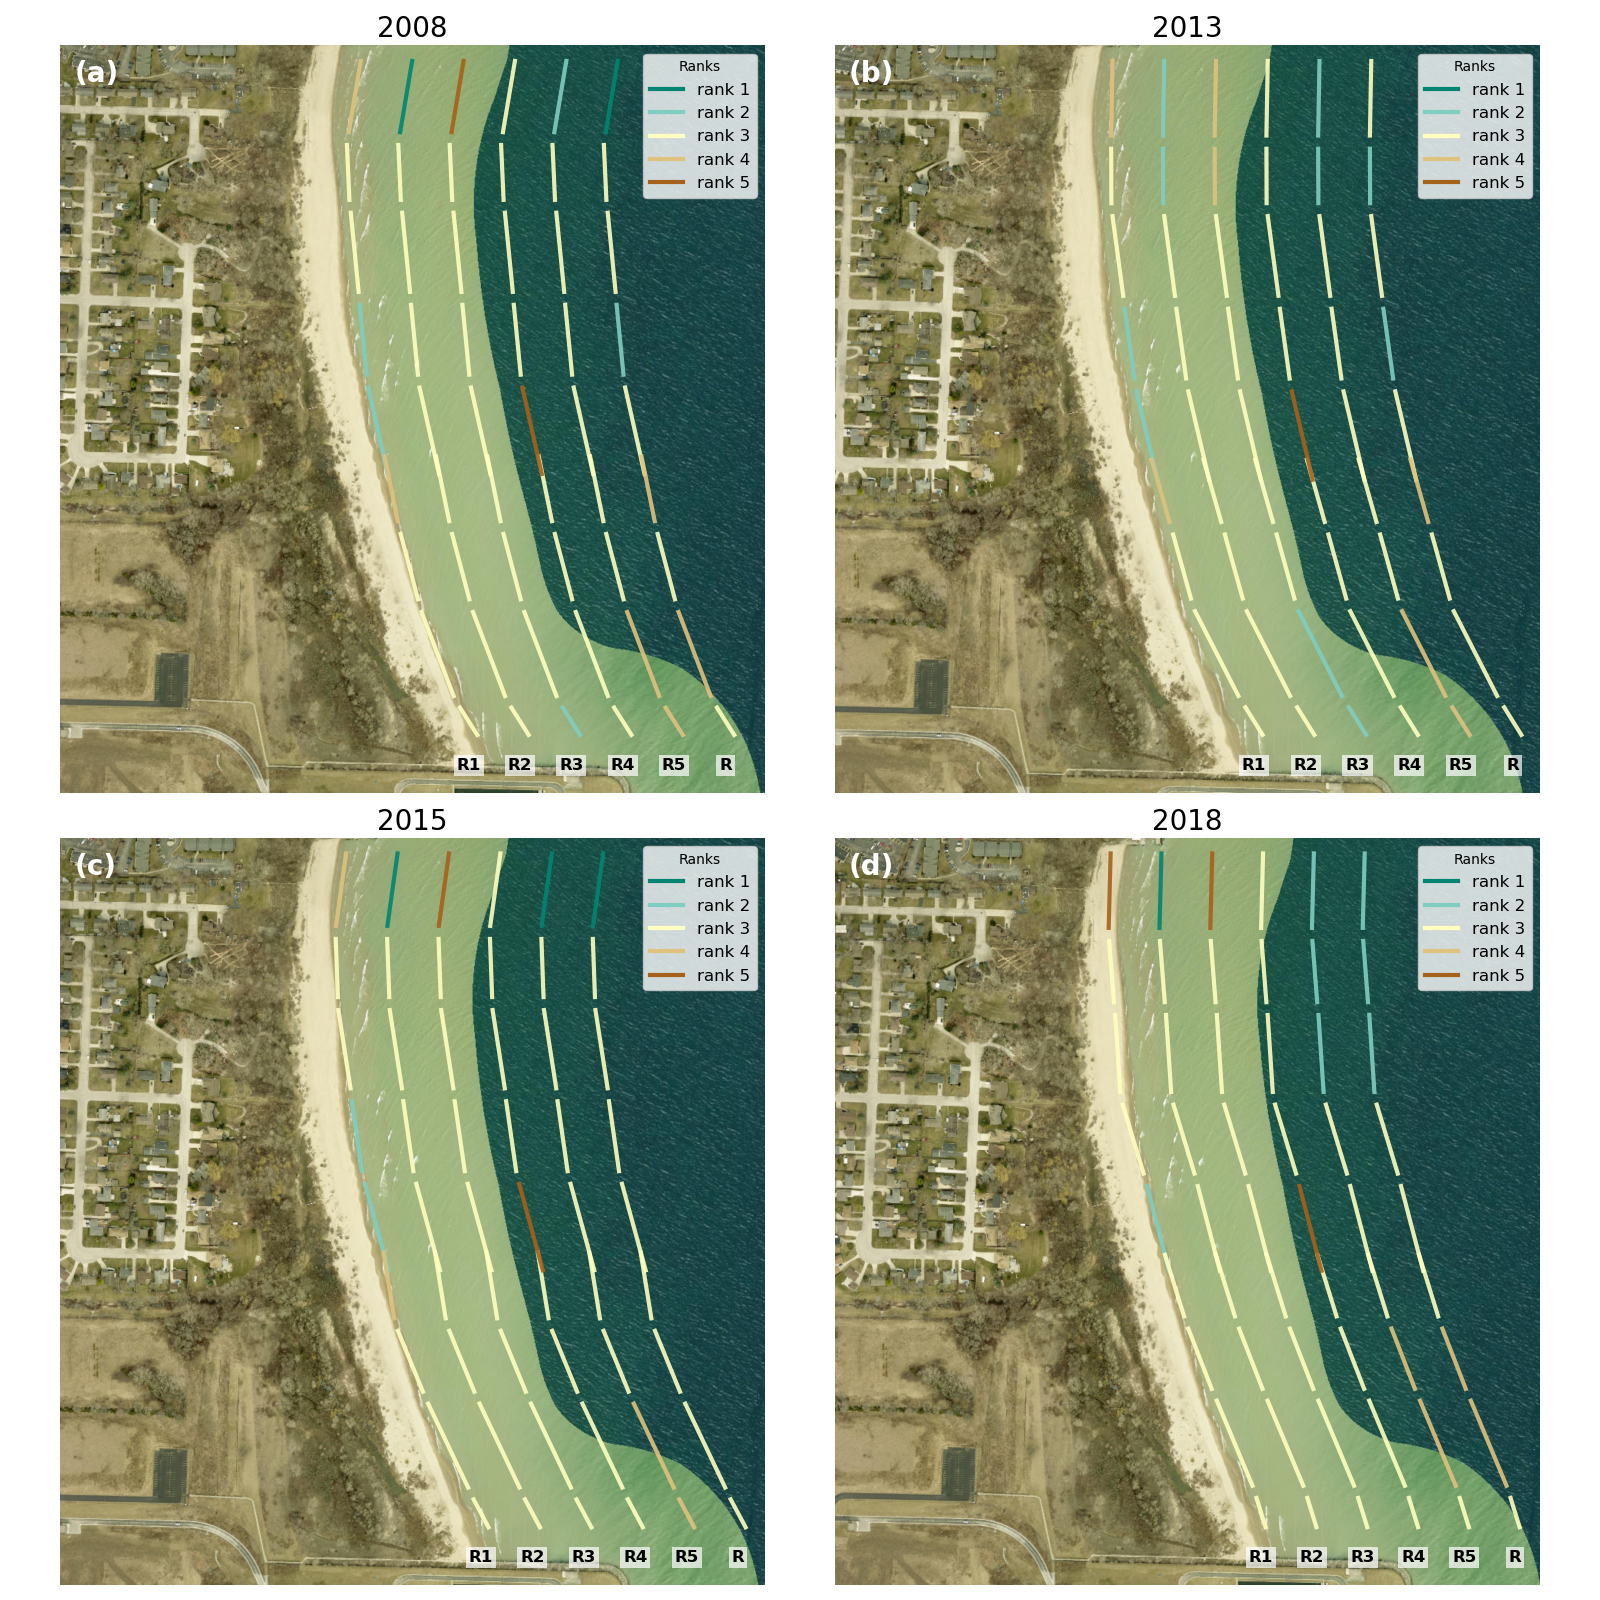
\includegraphics[width=1\textwidth]{chapter5/resources/site1_cvi.png}
  \caption{The ranks of vulnerability indicators in Oak Creek Beach.}
  \label{fig:s1_cv1}
\end{figure}

The vulnerability indicators for Oak Creek Beach are summarized in Table 5-2,
while the vulnerability ranks for each beach segment are presented in Figure
5-5. The RI indicates higher vulnerability ranks (rank 4) at the beach segment
2, 8, suggesting an increased likelihood of beach rotation. SEI does not exhibit
high vulnerability ranks across the beaches, with most of the ranks remaining
below 3. WHDI present a high vulnerability on the northern edge of the beach
(beach segment 8). The wave directionality in Oak Cree Beach is bidirectional
but northern wave dominant (see the wave rose in figure 5-2 b). The strong
northern wave tends to lead to rotation on the northern edge of the beach. LRI
has higher vulnerability in the middle of the beach (beach segment 4 and 5), due
to the steep beach slope measured in the middle of the beach slope. SBI presents
a higher vulnerability in the southern part of the beach (beach 2,3) and lower
vulnerability in the northern part (beach 2,3). The vulnerability caused by
sedimentation is significantly driven by the directionality of wave climate. The
longshore sediments are transported from the southern to northern that southern
edge of beach can be sediment starvation, indicating a large vulnerability. The
aggregated CVI for all five indicators is presented in Figure 5-6. The
distribution of the CVI is that the highest CVI appears in the middle of the
beach while the northern and southern edge of beaches tends to have lower
coastal vulnerability.

\subsection{Coastal vulnerability index at Whitting Lakefront Park}
\label{Coastal vulnerability index at Whitting Lakefront Park}

\begin{figure}[htbp]
  \centering
  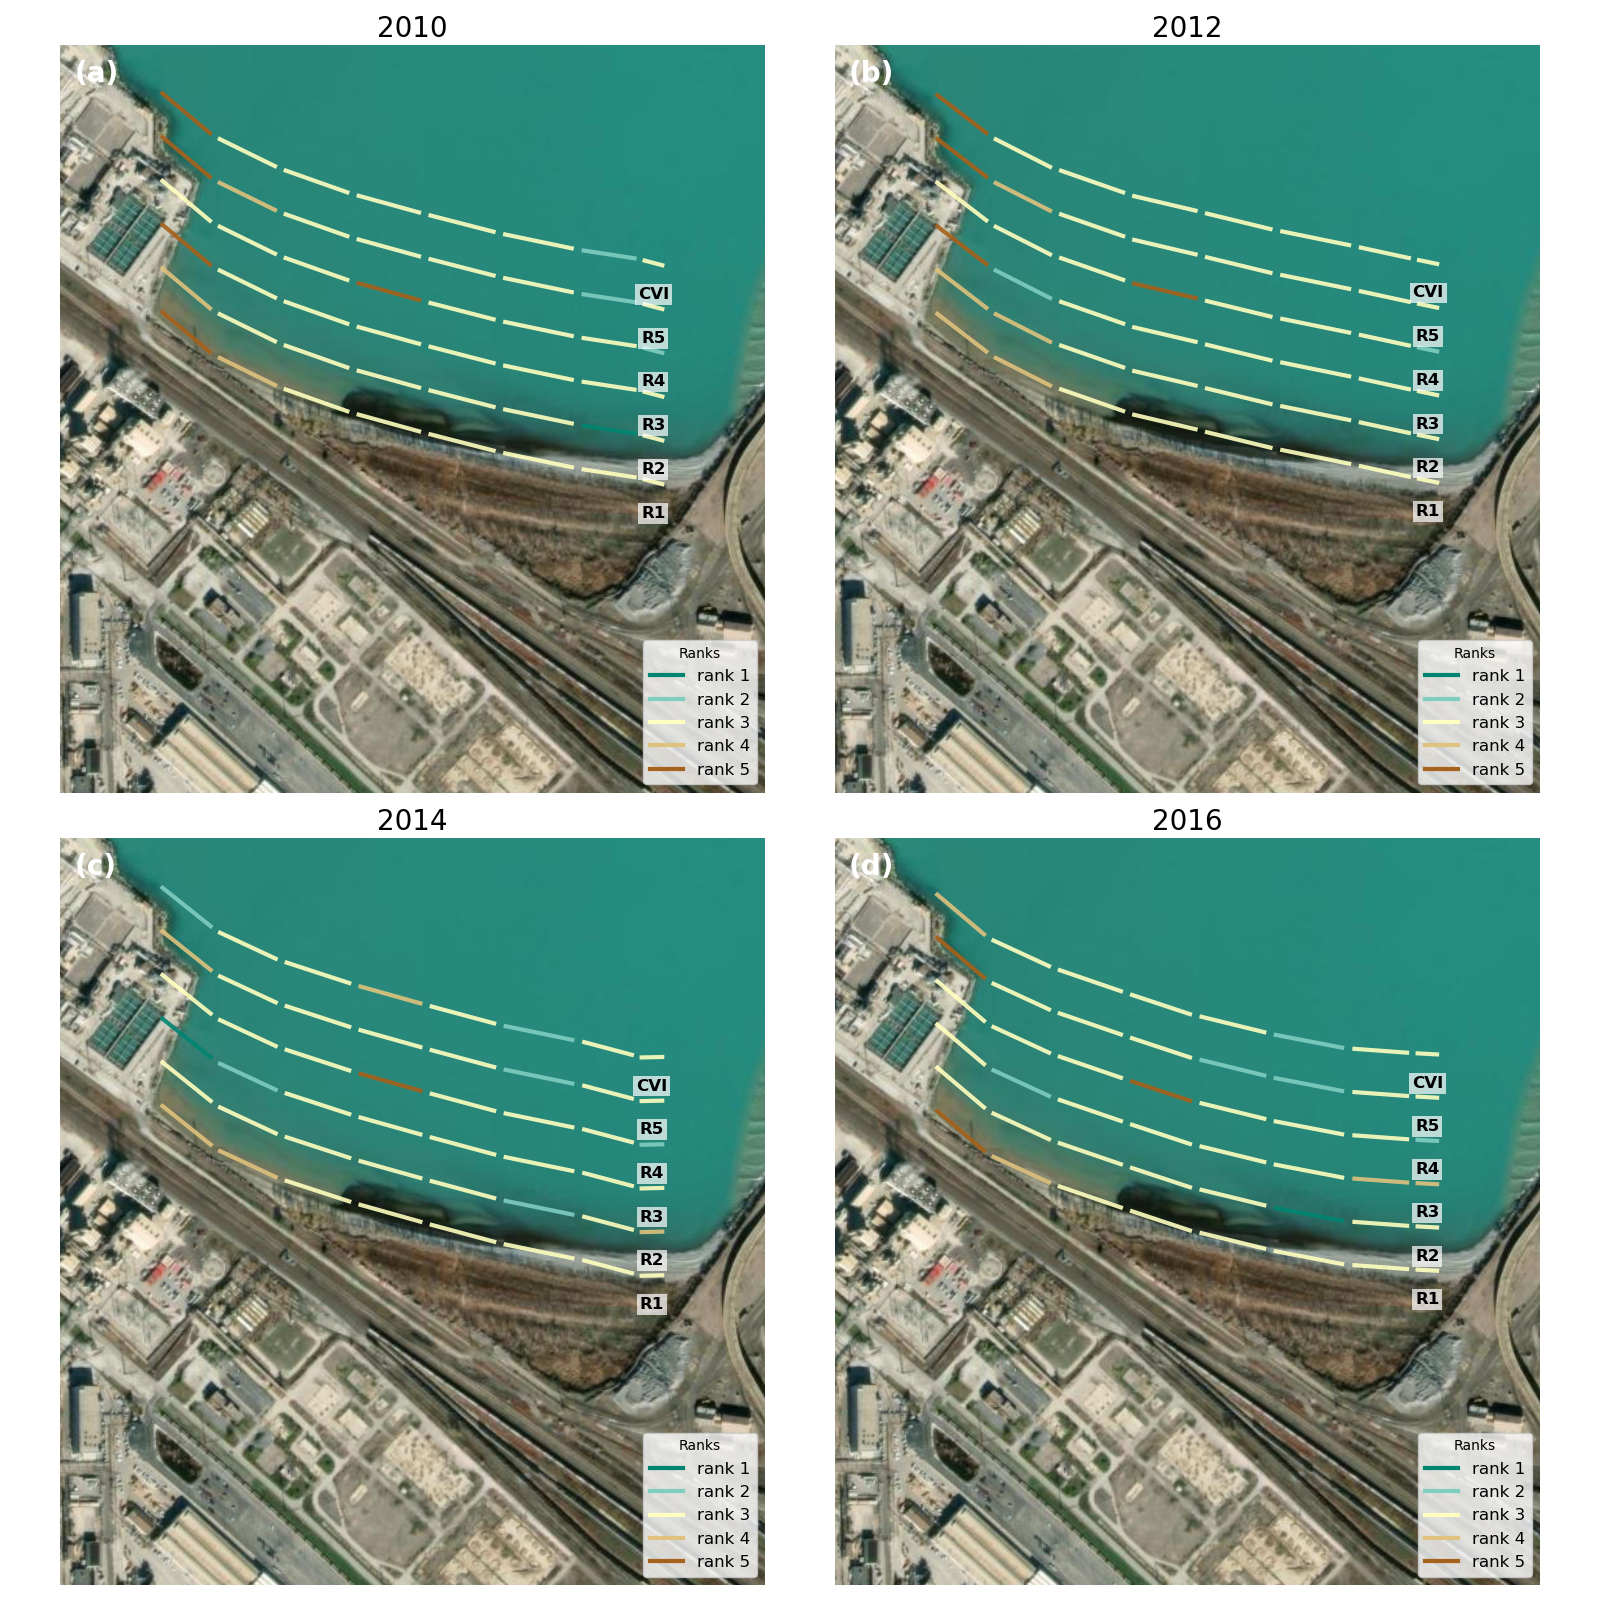
\includegraphics[width=1\textwidth]{chapter5/resources/site2_cvi.png}
  \caption{The ranks of vulnerability indicators in Whitting Beach.}
  \label{fig:s2_cv1}
\end{figure}

\subsection{Validation of CVI}
\label{Validation of CVI}

\begin{figure}[htbp]
  \centering
  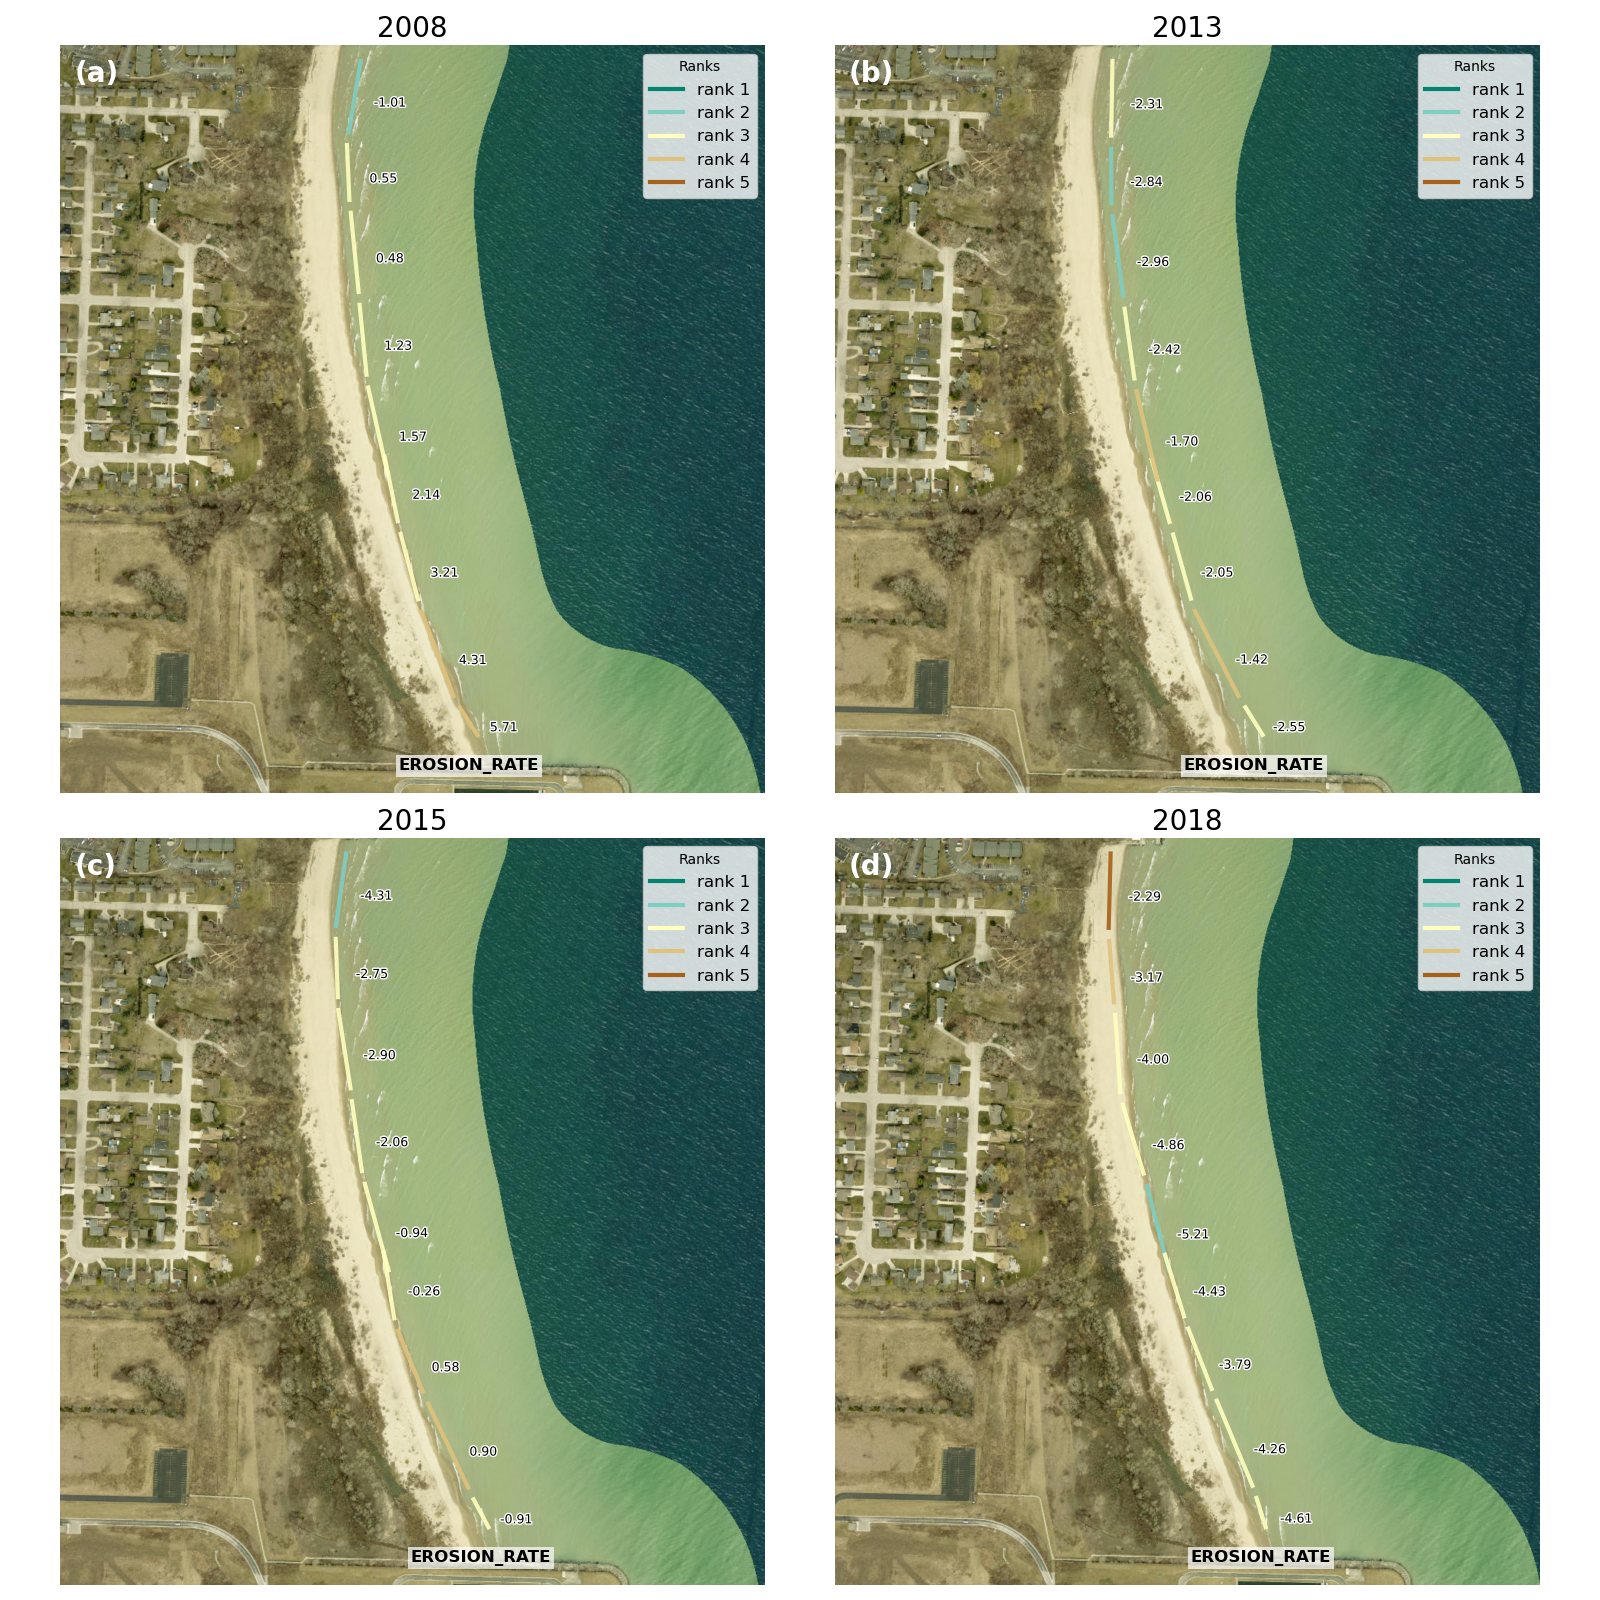
\includegraphics[width=1\textwidth]{chapter5/resources/site1_erosion.png}
  \caption{The shoreline erosion rates and corresponding ranks in Oak Creek Beach}
  \label{fig:s1_erosion}
\end{figure}

\begin{figure}[htbp]
  \centering
  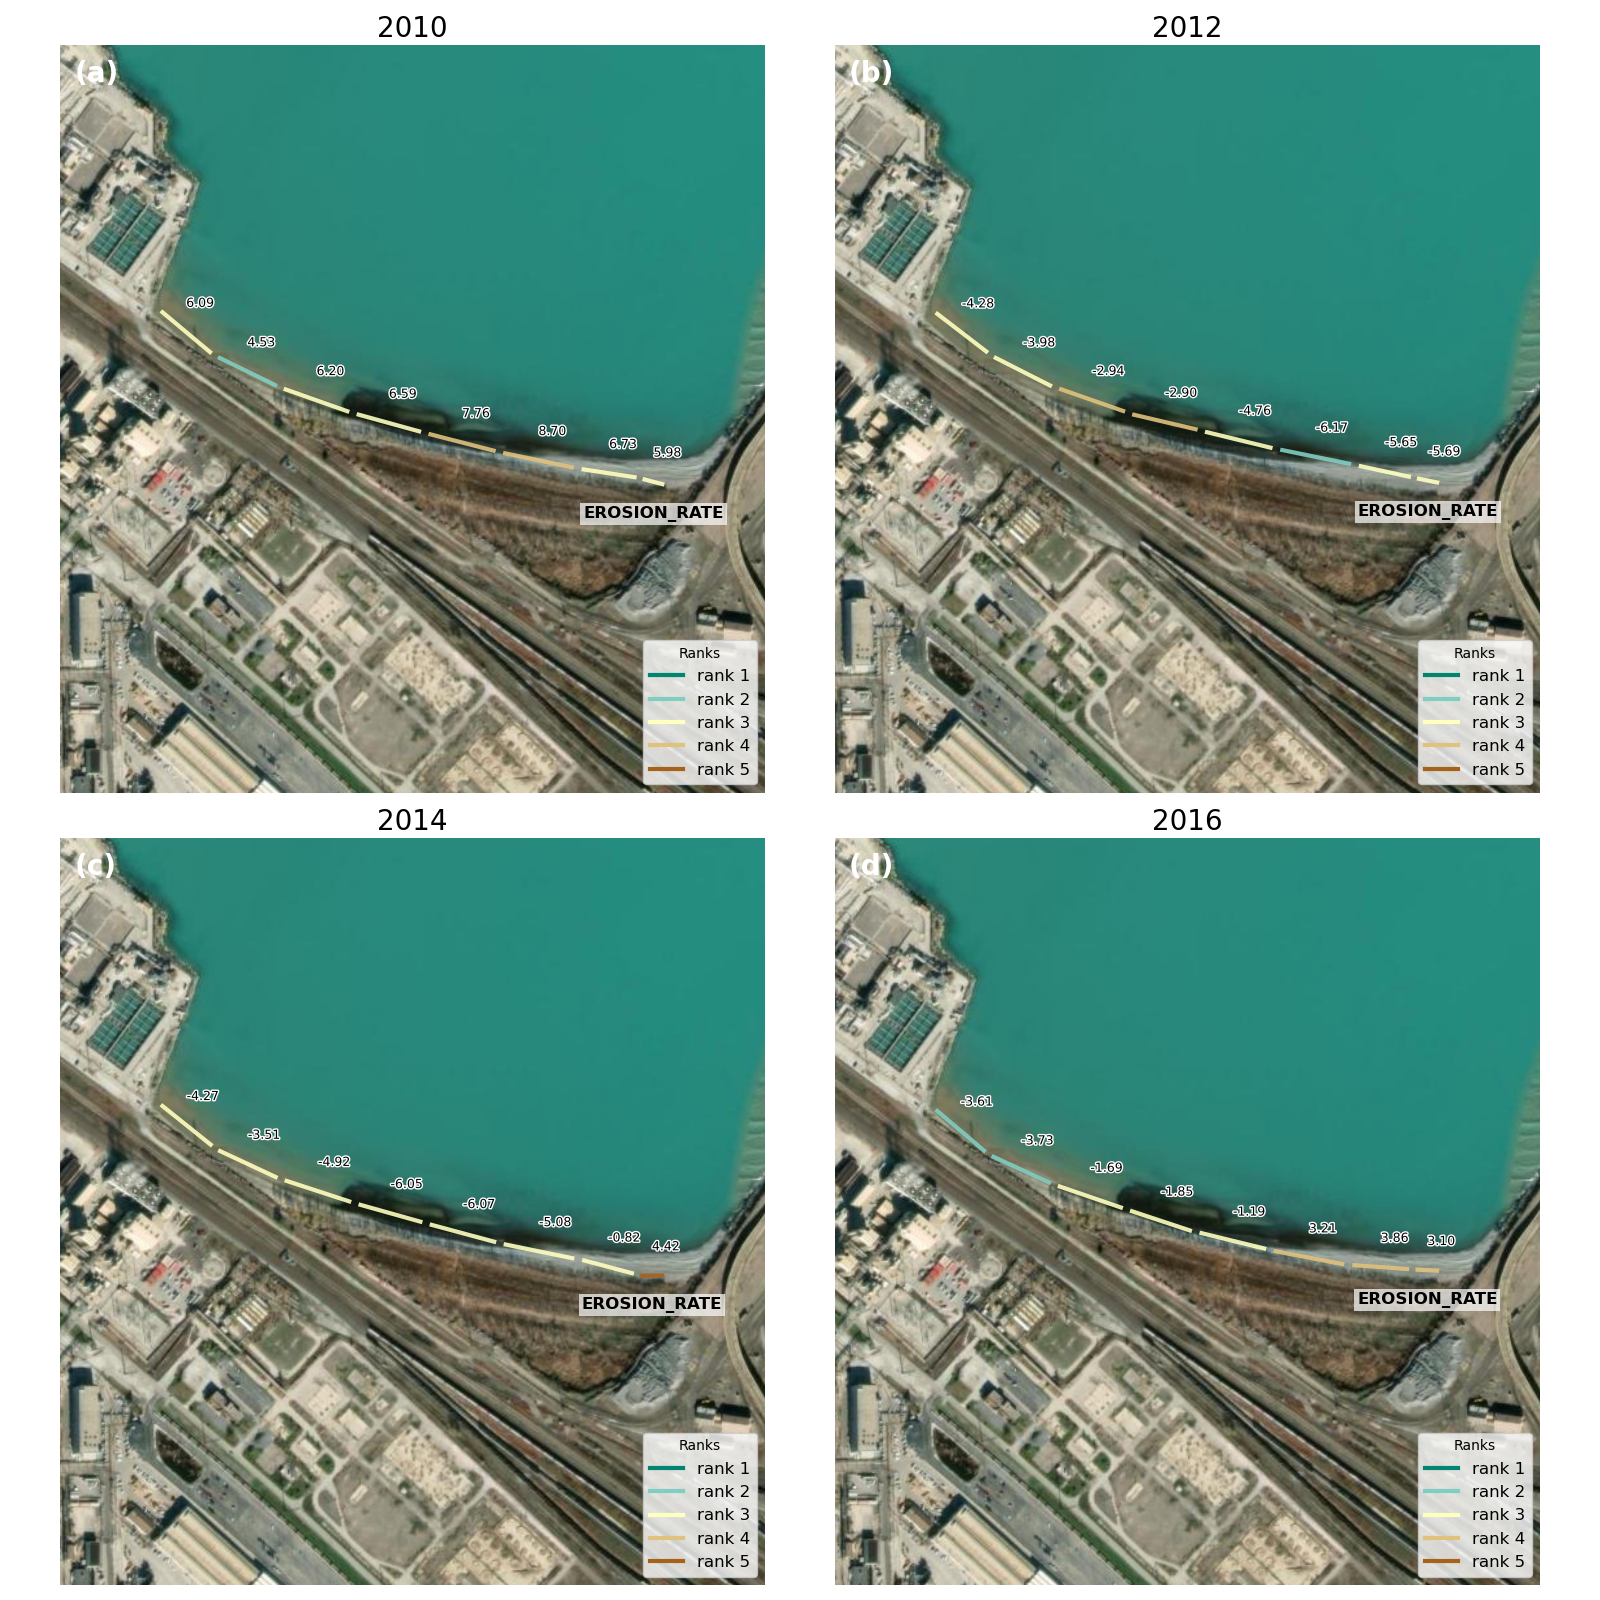
\includegraphics[width=1\textwidth]{chapter5/resources/site2_erosion.png}
  \caption{The shoreline erosion rates and corresponding ranks in Whitting Beach}
  \label{fig:s2_erosion}
\end{figure}

% Requires: \usepackage{booktabs}
\begin{table}[htbp]
\centering
\caption{Evaluation metrics for the Coastal Vulnerability Index (CVI) and its
subindices ($r_1$--$r_5$) against observed erosion-rate ranks (1--5) at Oak
Creek and Whitting Beach. Bold values indicate the best-performing subindex per
location for each metric.}
\label{tab:cvi_eval_oak_whitting}
\begin{tabular}{l l r r r r r}
\toprule
Location & Index & MAE & RMSE & QWK & $\rho$ & $\tau$ \\
\midrule
Oak Creek & CVI   & 0.694 & 1.067 & $-0.210$ & $-0.183$ & $-0.161$ \\
          & $R_1$ & 0.639 & 1.014 & $-0.114$ &  0.026 &  0.025 \\
          & $R_2$ & 0.500 & 0.943 & $-0.134$ & $-0.269$ & $-0.258$ \\
          & $R_3$ & \textbf{0.417} & \textbf{0.866} & \textbf{0.208} & \textbf{0.367} & \textbf{0.357} \\
          & $R_4$ & 0.556 & 0.943 &  0.053 &  0.050 &  0.048 \\
          & $R_5$ & 0.722 & 1.106 & $-0.294$ & $-0.340$ & $-0.324$ \\
\midrule
Whitting Beach & CVI   & 0.600 & 0.894 & 0.129 & 0.159 & 0.143 \\
               & $R_1$ & \textbf{0.525} & \textbf{0.822} & \textbf{0.289} & \textbf{0.393} & \textbf{0.367} \\
               & $R_2$ & 0.600 & 0.922 & $-0.071$ & $-0.103$ & $-0.093$ \\
               & $R_3$ & 0.700 & 1.049 & $-0.135$ & $-0.238$ & $-0.215$ \\
               & $R_4$ & 0.600 & 0.975 &  0.121 &  0.197 &  0.179 \\
               & $R_5$ & 0.600 & 0.866 &  0.236 &  0.250 &  0.225 \\
\bottomrule
\end{tabular}
\end{table}


\section{Discussions}
\label{c5_Discussions}

\subsection{Coefficient of CVI}
\label{Coefficient of CVI}

Although \citet{gornitz_global_1991} introduced the unweighted vulnerability index,
which is presented in \ref{eq:eq5.6}, it is not an accurate approach for evaluation goal,
as all component of subindices sharing equal weights \citet{fu2022characteristics}. A common
adaptation of it is to apply a weighted index with summation.
\begin{equation}
  CVI_{weighted} = \sum_{i=1}^{n}W_ir_i
\label{eq:eq5.7}
\end{equation}

\begin{table}[htbp]
\centering
\caption{Performance metrics and weights for Whitting Beach and Oak Creek Beach}
\label{tab:whitting_oakcreek_vertical}
\setlength{\tabcolsep}{4pt} % reduce horizontal padding
\renewcommand{\arraystretch}{1.1} % tighter rows
\begin{tabular}{p{2.0cm} c c c c c c c c c c}
\toprule
Site & $\alpha$ & MAE & QWK & SpearmanR & KendallTau & $w_1$ & $w_2$ & $w_3$ & $w_4$ & $w_5$ \\
\midrule
\multirow{5}{=}{\raggedright Whitting\\Beach}
 & 0.00 & 1.583 & -0.121 & -0.223 & -0.196 & 0.101 & 0.034 & 0.063 & 0.775 & 0.027 \\
 & 0.25 & 1.417 &  0.011 & -0.031 & -0.027 & 0.126 & 0.075 & 0.097 & 0.631 & 0.070 \\
 & 0.50 & 1.389 &  0.096 &  0.102 &  0.091 & 0.151 & 0.117 & 0.132 & 0.487 & 0.114 \\
 & 0.75 & 1.389 &  0.096 &  0.102 &  0.091 & 0.176 & 0.158 & 0.166 & 0.344 & 0.157 \\
 & 1.00 & 1.194 &  0.099 &  0.113 &  0.096 & 0.200 & 0.200 & 0.200 & 0.200 & 0.200 \\
\midrule
\multirow{5}{=}{\raggedright Oak Creek\\Beach}
 & 0.00 & 1.550 & -0.184 & -0.255 & -0.222 & 0.717 & 0.033 & 0.031 & 0.115 & 0.104 \\
 & 0.25 & 1.550 & -0.184 & -0.255 & -0.222 & 0.587 & 0.075 & 0.073 & 0.136 & 0.128 \\
 & 0.50 & 1.550 & -0.184 & -0.255 & -0.222 & 0.458 & 0.117 & 0.116 & 0.157 & 0.152 \\
 & 0.75 & 1.525 & -0.186 & -0.257 & -0.225 & 0.329 & 0.158 & 0.158 & 0.179 & 0.176 \\
 & 1.00 & 1.625 & -0.056 & -0.043 & -0.037 & 0.200 & 0.200 & 0.200 & 0.200 & 0.200 \\
\bottomrule
\end{tabular}
\end{table}




\subsection{Coastal vulnerability and beach rotation}
\label{rotation}

\begin{figure}[htbp]
  \centering
  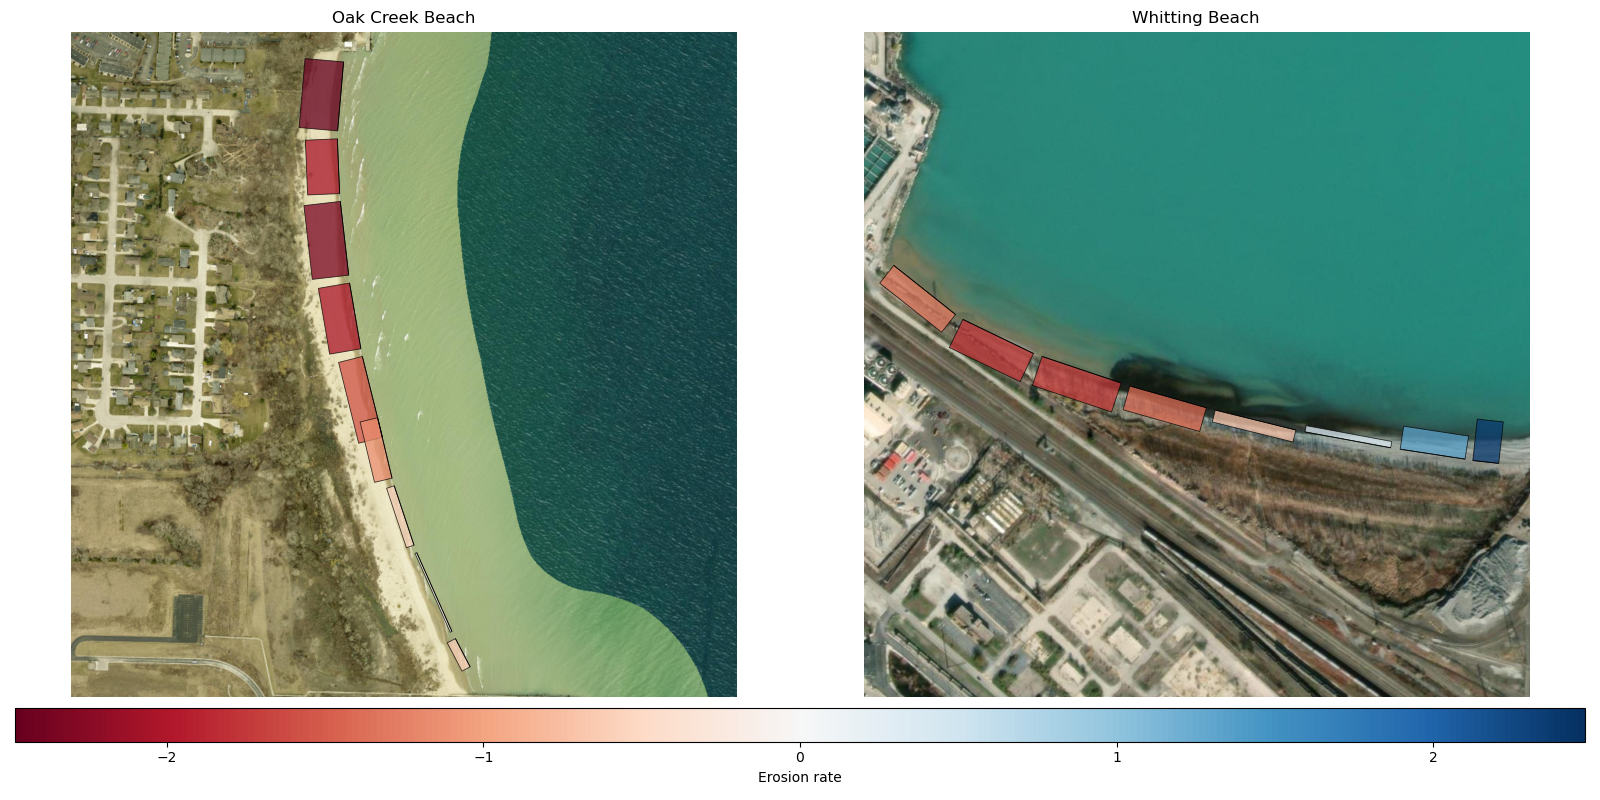
\includegraphics[width=1\textwidth]{chapter5/resources/sites_rotation.png}
  \caption{Beach rotations in two sites. (a) Oak Creek Beach (b) Whitting beach}
  \label{fig:cites_rotations}
\end{figure}

\subsection{Limitation of CVI and future works}
\label{Limitation of CVI}

\section{Conclusion}
\label{c5_Conclusion}